\documentclass{article} 
\usepackage{graphicx}
\usepackage{caption}
\usepackage{subcaption}
\title{Report for Home Problem 2, FFR105}
\author{Jesper Persson - 9008040199}
\begin{document} 
\maketitle

\section{2.1}

\subsection{a}

Starting from a city, we will have N-1 options of where to go next, and from the next city, we will have N-2 options, and so on, until there is only 1 city to chose. This will give us N-1 * N-2 *...1, or (N-1)! paths in total. However, to find only the distinct paths, we now need to eliminate the duplicates. For each path, we know we can can find the same (distinct) path by simply reversing it. Thus, (N-1)! will contain twice as many paths as we want, and the answer is that there are (N-1)! / 2 distinctive paths between the N cities.

\subsection{b-d}

\begin{figure}[!ht]
        \centering
        \begin{subfigure}[b]{0.3\textwidth}
                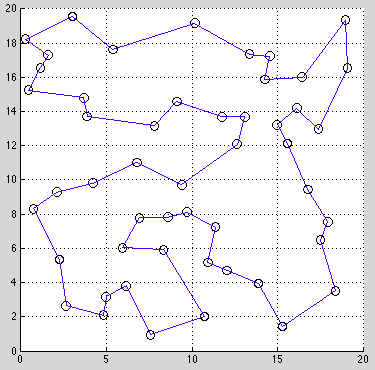
\includegraphics[width=\textwidth]{AC}
                \caption{Ant Colony - Length 121.1}
                \label{fig:Ant}
        \end{subfigure}
        \begin{subfigure}[b]{0.3\textwidth}
                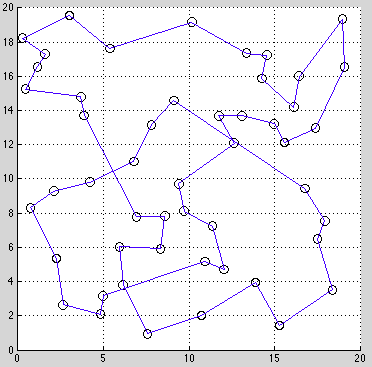
\includegraphics[width=\textwidth]{21b}
                \caption{GA, random start - Length 134.92}
                \label{fig:GA-random}
        \end{subfigure}
        \begin{subfigure}[b]{0.3\textwidth}
                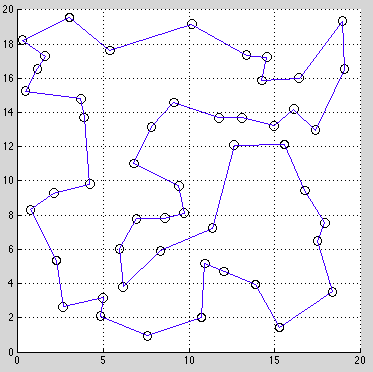
\includegraphics[width=\textwidth]{21d}
                \caption{GA, NN start - Length 124.53}
                \label{fig:GA-NN}
        \end{subfigure}
        \caption{Paths of the different algorithms}\label{fig:algorithms}
\end{figure}

The best path was found by the Ant Colony, and is include	d in the file "GetBestPath.m".
\newpage

\section{2.2}
\end{document}